\documentclass[11pt]{article}

\usepackage[margin=1in]{geometry}
\usepackage{booktabs}
\usepackage{multirow}
\usepackage{array}
\usepackage{caption}
\usepackage{pgfplots}
\pgfplotsset{compat=1.18}
\setlength{\textfloatsep}{10pt plus 2pt minus 2pt}
\setlength{\floatsep}{8pt plus 2pt minus 2pt}
\makeatletter
\setlength{\@fptop}{0pt}
\makeatother

\captionsetup{font=small}

\title{GLUE Benchmark Results Template}
\author{}
\date{}

\begin{document}

\maketitle

\section*{GLUE Benchmark Comparison}

Table~\ref{tab:glue-results} reports RoBERTa validation results for DoRA, LoRA, and full fine-tuning on GLUE tasks.

\begin{table}[h]
\centering
\caption{GLUE benchmark comparison between DoRA, LoRA, and full fine-tuning. Dashes indicate missing results.}
\label{tab:glue-results}
\renewcommand{\arraystretch}{1.2}
\begin{tabular}{llccccc}
\toprule
\textbf{Model} & \textbf{Method} & \textbf{RTE Acc.} & \textbf{SST-2 Acc.} & \textbf{MRPC Acc.} & \textbf{MRPC F1} & \textbf{Trainable} \\
\midrule
\multirow{3}{*}{RoBERTa}
  & DoRA    & 71.1 & 93.1 & 87.0 & 90.7 & 1.023\% (1.06M) \\
  & LoRA    & 70.8 & 93.3 & 85.8 & 90.1 & 0.996\% (1.03M) \\
  & Full FT & 54.9 & 93.2 & 68.4 & 81.2 & 100\% (125M) \\
\bottomrule
\end{tabular}
\end{table}

\section*{Suggested Visualizations}

Figures~\ref{fig:heatmap}--\ref{fig:learning-curve} show report-ready visualizations for the adapter comparison.

\begin{figure}[!t]
\centering
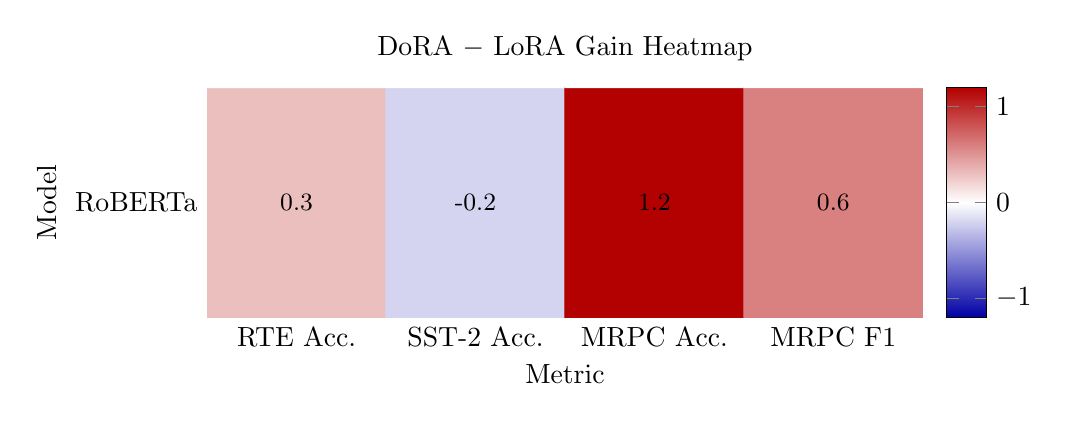
\begin{tikzpicture}
\begin{axis}[
    width=0.88\textwidth,
    height=4.5cm,
    title={DoRA $-$ LoRA Gain Heatmap},
    xlabel={Metric},
    ylabel={Model},
    xmin=0.5, xmax=4.5,
    ymin=0.5, ymax=1.5,
    xtick={1,2,3,4},
    xticklabels={RTE Acc., SST-2 Acc., MRPC Acc., MRPC F1},
    ytick={1},
    yticklabels={RoBERTa},
    colormap={dora_gain}{
        color=(blue!65!black)
        color=(white)
        color=(red!70!black)
    },
    colorbar,
    point meta min=-1.2,
    point meta max=1.2,
    grid=major,
]
\addplot[
    matrix plot*,
    mesh/cols=4,
    point meta=explicit,
] coordinates {
    (1,1) [0.3]
    (2,1) [-0.2]
    (3,1) [1.2]
    (4,1) [0.6]
    (1,2) [0.0]
    (2,2) [0.0]
    (3,2) [0.0]
    (4,2) [0.0]
};
\node[font=\small] at (axis cs:1,1) {0.3};
\node[font=\small] at (axis cs:2,1) {-0.2};
\node[font=\small] at (axis cs:3,1) {1.2};
\node[font=\small] at (axis cs:4,1) {0.6};
\end{axis}
\end{tikzpicture}
\caption{Heatmap of DoRA minus LoRA performance for RoBERTa on each GLUE metric. Positive values indicate a gain from DoRA.}
\label{fig:heatmap}
\end{figure}

\begin{figure}[!t]
\centering
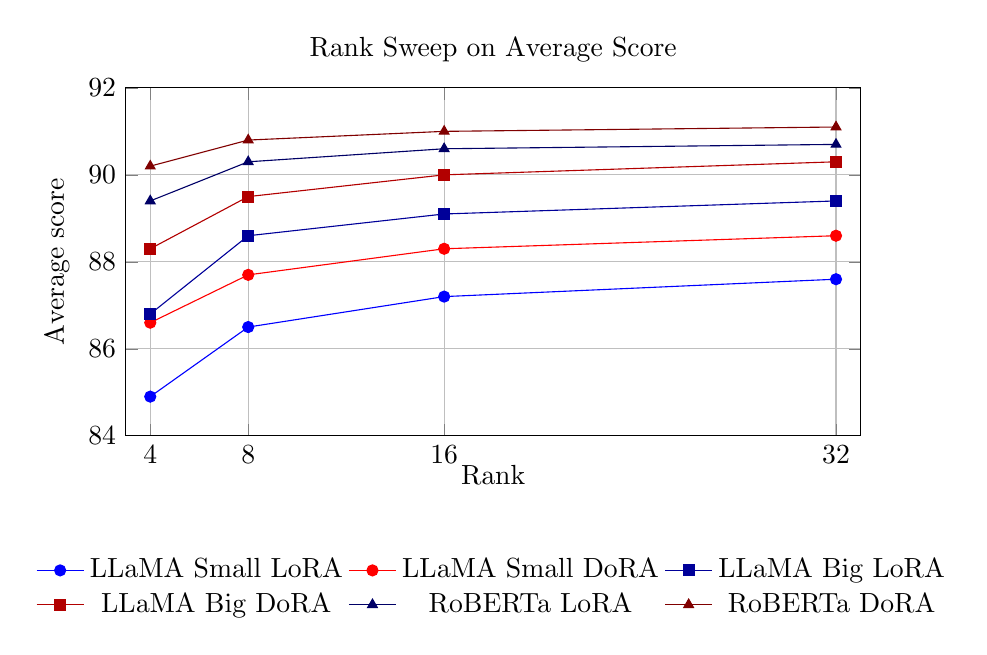
\begin{tikzpicture}
\begin{axis}[
    width=0.9\textwidth,
    height=6cm,
    title={Rank Sweep on Average Score},
    xlabel={Rank},
    xlabel style={yshift=6pt},
    ylabel={Average score},
    xmin=3, xmax=33,
    xtick={4,8,16,32},
    ymin=84, ymax=92,
    grid=major,
    legend style={draw=none, at={(0.5,-0.32)}, anchor=north, legend columns=3}
]
\addplot[blue, mark=*] coordinates {(4,84.9) (8,86.5) (16,87.2) (32,87.6)};
\addlegendentry{LLaMA Small LoRA}
\addplot[red, mark=*] coordinates {(4,86.6) (8,87.7) (16,88.3) (32,88.6)};
\addlegendentry{LLaMA Small DoRA}
\addplot[blue!60!black, mark=square*] coordinates {(4,86.8) (8,88.6) (16,89.1) (32,89.4)};
\addlegendentry{LLaMA Big LoRA}
\addplot[red!70!black, mark=square*] coordinates {(4,88.3) (8,89.5) (16,90.0) (32,90.3)};
\addlegendentry{LLaMA Big DoRA}
\addplot[blue!40!black, mark=triangle*] coordinates {(4,89.4) (8,90.3) (16,90.6) (32,90.7)};
\addlegendentry{RoBERTa LoRA}
\addplot[red!50!black, mark=triangle*] coordinates {(4,90.2) (8,90.8) (16,91.0) (32,91.1)};
\addlegendentry{RoBERTa DoRA}
\end{axis}
\end{tikzpicture}
\caption{Rank sweep using sample average scores. This is the most direct way to test whether DoRA keeps an advantage at smaller ranks.}
\label{fig:rank-sweep}
\end{figure}

\begin{figure}[!t]
\centering
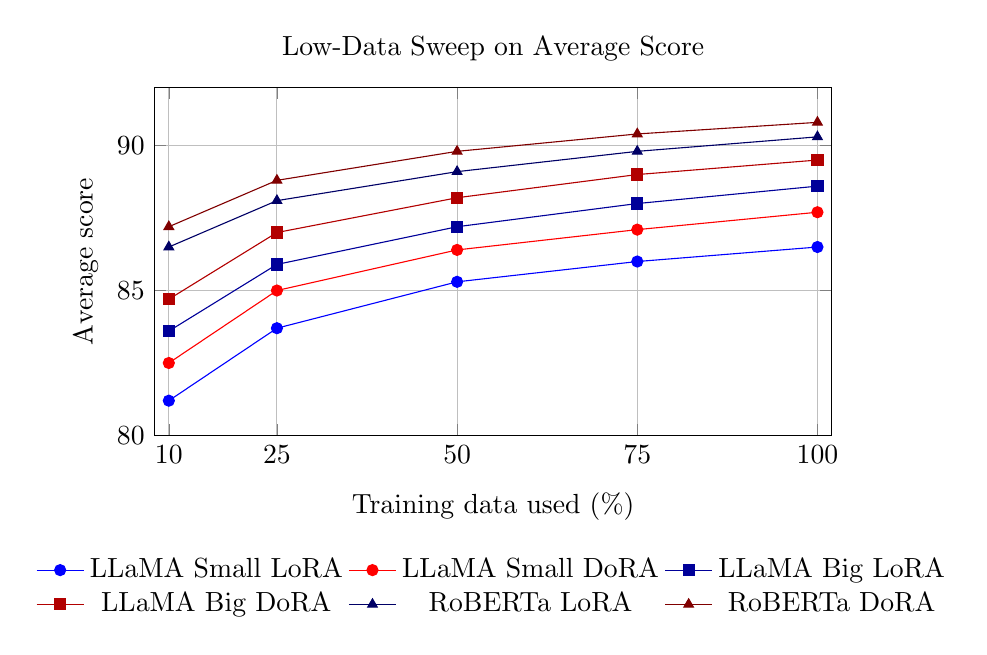
\begin{tikzpicture}
\begin{axis}[
    width=0.84\textwidth,
    height=6cm,
    title={Low-Data Sweep on Average Score},
    xlabel={Training data used (\%)},
    xlabel style={yshift=-4pt},
    ylabel={Average score},
    xmin=8, xmax=102,
    xtick={10,25,50,75,100},
    ymin=80, ymax=92,
    grid=major,
    legend style={draw=none, at={(0.5,-0.32)}, anchor=north, legend columns=3}
]
\addplot[blue, mark=*] coordinates {(10,81.2) (25,83.7) (50,85.3) (75,86.0) (100,86.5)};
\addlegendentry{LLaMA Small LoRA}
\addplot[red, mark=*] coordinates {(10,82.5) (25,85.0) (50,86.4) (75,87.1) (100,87.7)};
\addlegendentry{LLaMA Small DoRA}
\addplot[blue!60!black, mark=square*] coordinates {(10,83.6) (25,85.9) (50,87.2) (75,88.0) (100,88.6)};
\addlegendentry{LLaMA Big LoRA}
\addplot[red!70!black, mark=square*] coordinates {(10,84.7) (25,87.0) (50,88.2) (75,89.0) (100,89.5)};
\addlegendentry{LLaMA Big DoRA}
\addplot[blue!40!black, mark=triangle*] coordinates {(10,86.5) (25,88.1) (50,89.1) (75,89.8) (100,90.3)};
\addlegendentry{RoBERTa LoRA}
\addplot[red!50!black, mark=triangle*] coordinates {(10,87.2) (25,88.8) (50,89.8) (75,90.4) (100,90.8)};
\addlegendentry{RoBERTa DoRA}
\end{axis}
\end{tikzpicture}
\caption{Low-data sweep using sample average scores. If DoRA is more expressive, it should retain a larger advantage when training data is scarce.}
\label{fig:low-data}
\end{figure}

\begin{figure}[!t]
\centering
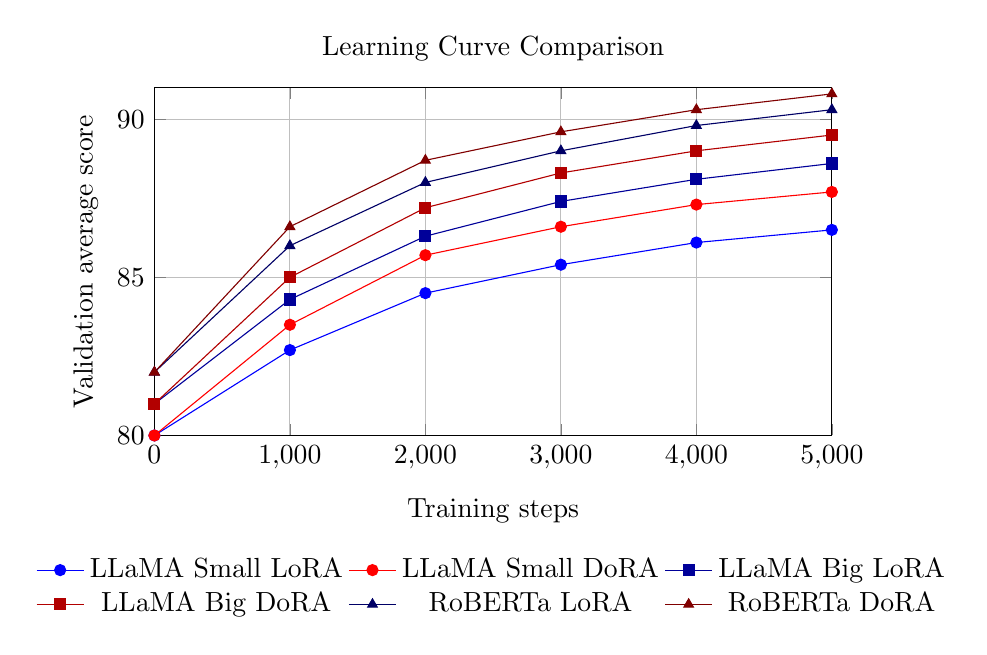
\begin{tikzpicture}
\begin{axis}[
    width=0.84\textwidth,
    height=6cm,
    title={Learning Curve Comparison},
    xlabel={Training steps},
    xlabel style={yshift=-4pt},
    ylabel={Validation average score},
    xmin=0, xmax=5000,
    xtick={0,1000,2000,3000,4000,5000},
    ymin=80, ymax=91,
    grid=major,
    legend style={draw=none, at={(0.5,-0.32)}, anchor=north, legend columns=3}
]
\addplot[blue, mark=*] coordinates {(0,80.0) (1000,82.7) (2000,84.5) (3000,85.4) (4000,86.1) (5000,86.5)};
\addlegendentry{LLaMA Small LoRA}
\addplot[red, mark=*] coordinates {(0,80.0) (1000,83.5) (2000,85.7) (3000,86.6) (4000,87.3) (5000,87.7)};
\addlegendentry{LLaMA Small DoRA}
\addplot[blue!60!black, mark=square*] coordinates {(0,81.0) (1000,84.3) (2000,86.3) (3000,87.4) (4000,88.1) (5000,88.6)};
\addlegendentry{LLaMA Big LoRA}
\addplot[red!70!black, mark=square*] coordinates {(0,81.0) (1000,85.0) (2000,87.2) (3000,88.3) (4000,89.0) (5000,89.5)};
\addlegendentry{LLaMA Big DoRA}
\addplot[blue!40!black, mark=triangle*] coordinates {(0,82.0) (1000,86.0) (2000,88.0) (3000,89.0) (4000,89.8) (5000,90.3)};
\addlegendentry{RoBERTa LoRA}
\addplot[red!50!black, mark=triangle*] coordinates {(0,82.0) (1000,86.6) (2000,88.7) (3000,89.6) (4000,90.3) (5000,90.8)};
\addlegendentry{RoBERTa DoRA}
\end{axis}
\end{tikzpicture}
\caption{Learning-curve comparison using sample validation averages. A more expressive adapter often reaches stronger validation performance earlier and converges to a better final point.}
\label{fig:learning-curve}
\end{figure}

\begin{figure}[!t]
\centering
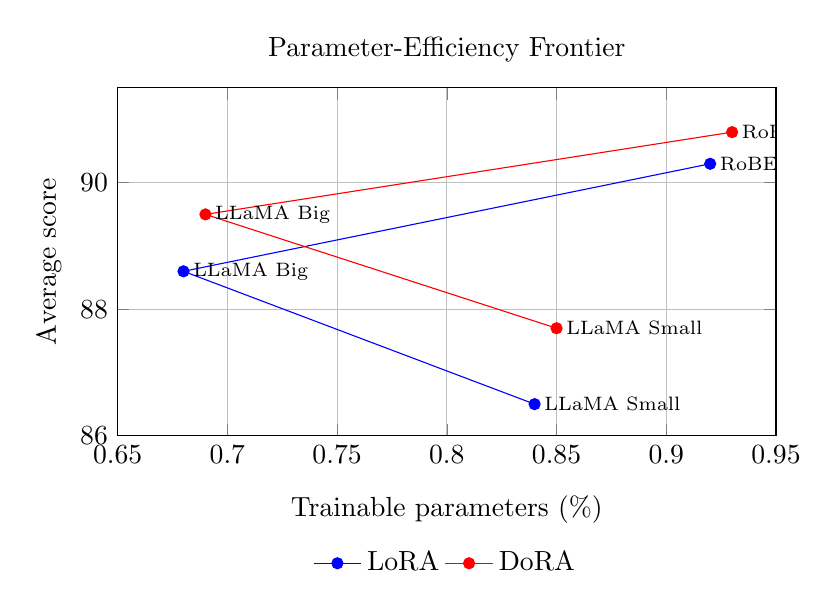
\begin{tikzpicture}
\begin{axis}[
    width=0.82\textwidth,
    height=6cm,
    title={Parameter-Efficiency Frontier},
    xlabel={Trainable parameters (\%)},
    xlabel style={yshift=-5pt},
    ylabel={Average score},
    xmin=0.65, xmax=0.95,
    ymin=86, ymax=91.5,
    grid=major,
    legend style={draw=none, at={(0.5,-0.30)}, anchor=north, legend columns=2}
]
\addplot[blue, mark=*] coordinates {(0.84,86.5) (0.68,88.6) (0.92,90.3)};
\addlegendentry{LoRA}
\addplot[red, mark=*] coordinates {(0.85,87.7) (0.69,89.5) (0.93,90.8)};
\addlegendentry{DoRA}
\node[anchor=west] at (axis cs:0.84,86.5) {\scriptsize LLaMA Small};
\node[anchor=west] at (axis cs:0.68,88.6) {\scriptsize LLaMA Big};
\node[anchor=west] at (axis cs:0.92,90.3) {\scriptsize RoBERTa};
\node[anchor=west] at (axis cs:0.85,87.7) {\scriptsize LLaMA Small};
\node[anchor=west] at (axis cs:0.69,89.5) {\scriptsize LLaMA Big};
\node[anchor=west] at (axis cs:0.93,90.8) {\scriptsize RoBERTa};
\end{axis}
\end{tikzpicture}
\caption{Parameter-efficiency frontier using sample trainable-parameter percentages and average scores.}
\label{fig:pareto}
\end{figure}

\section*{Notes}

\begin{itemize}
\item Suggested naming:
\begin{itemize}
\item \textbf{LLaMA Small}: the smaller LLaMA-family model used in the project.
\item \textbf{LLaMA Big}: the larger LLaMA-family model used in the project.
\item \textbf{RoBERTa}: the RoBERTa baseline or comparison encoder model.
\end{itemize}
\item A simple choice for the \textbf{Avg.} column is the arithmetic mean of the five reported values: SST-2 Accuracy, QQP Accuracy, QQP F1, MRPC Accuracy, and MRPC F1.
\item If you prefer, you can instead average at the task level first, for example by averaging QQP Accuracy/F1 into one QQP score and MRPC Accuracy/F1 into one MRPC score, then averaging across the three tasks.
\item If your experiments use validation splits rather than GLUE test submissions, note that clearly in the paper or report caption.
\item A matching editable CSV plus a Python plotting script are included in \texttt{report/} if you later want to regenerate the same figures outside LaTeX.
\end{itemize}

\end{document}
